\section{Metodologías usadas}
\label{Metodologias usadas}

    La guía SWEBOK (\emph{Software Engineering Body of Knowledge}) \cite{SWEBOK2014} divide la ingeniería del software en procesos disciplinados para planificar, ejecutar y controlar el desarrollo frente a restricciones reales. Elegir un método de trabajo determina cómo evoluciona el código y cómo se responde a cambios en los requisitos sin comprometer la estabilidad del sistema.

\subsection{Revisión de enfoques metodológicos}

    El modelo tradicional en cascada exige completar y congelar cada fase antes de iniciar la siguiente: requisitos, diseño, codificación, verificación y entrega. Si bien funciona en proyectos con especificaciones cerradas y contratos rígidos, fracasa al integrar servicios desacoplados o protocolos emergentes como MCP. Descubrir un fallo de integración en la fase final de pruebas dispararía el coste de rehacer módulos enteros.

    Scrum estructura el trabajo en iteraciones cortas llamadas \emph{sprints}, orientadas a entregar incrementos funcionales cada dos o cuatro semanas. Reparte responsabilidades entre perfiles definidos (\emph{Scrum Master}, \emph{Product Owner}, equipo de desarrollo) y exige reuniones periódicas de sincronización y retrospectiva. Pese a dominar en la industria corporativa, su burocracia de reuniones pierde sentido en un proyecto individual sin equipo que coordinar. La figura \ref{fig:agile_vs_waterfall} refleja la comparativa histórica de tasas de éxito entre ambos enfoques.

\begin{figure}[H]
    \centering
    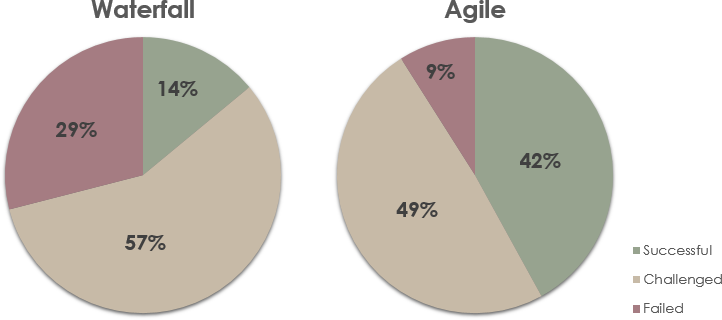
\includegraphics[width=0.68\textwidth]{HerramientasYMetodologias/img/Waterfall_vs_agile.png}
    \caption{Diferencia de éxito entre metodologías ágiles y tradicionales en cascada}
    \label{fig:agile_vs_waterfall}
\end{figure}

    Kanban elimina las cadencias temporales fijas y se centra en limitar el trabajo en curso o WIP (\emph{Work In Progress}). Las tareas avanzan a través de columnas de estado en un tablero visual (figura \ref{fig:tablero_kanban}): pendientes, en desarrollo y completadas. Este flujo continuo permite priorizar el trabajo según cuellos de botella reales, facilitando al programador concentrarse en un solo componente hasta cerrarlo.

\begin{figure}[H]
    \centering
    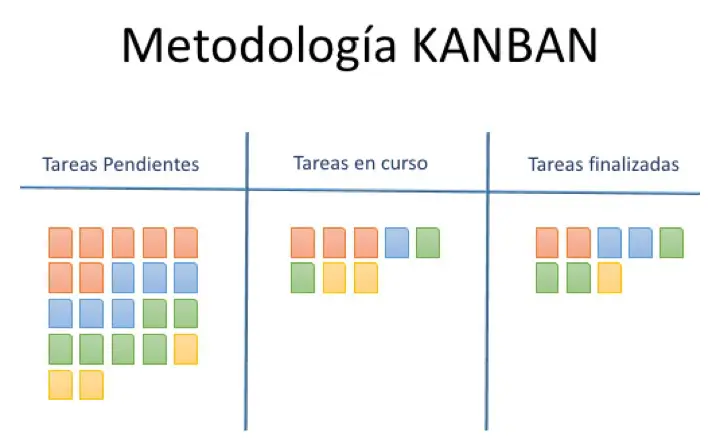
\includegraphics[width=0.68\textwidth]{HerramientasYMetodologias/img/Kanban.png}
    \caption{Tablero Kanban representativo del flujo de desarrollo ágil}
    \label{fig:tablero_kanban}
\end{figure}

    La programación extrema (\emph{Extreme Programming} o XP) antepone la excelencia en el código a la gestión burocrática. Sus pilares incluyen la refactorización continua, la integración frecuente y el desarrollo guiado por pruebas o TDD (\emph{Test-Driven Development}). En TDD, los tests se redactan antes que el código de producción, garantizando que cada función responda a una necesidad validada y medible.

\subsection{Análisis comparativo y selección para el proyecto}

    La arquitectura de Colivi —un backend modular en Spring Boot 3, un servidor MCP independiente en Node.js, un cliente web en React y el paquete móvil con Capacitor— hacía inviable una cascada estricta. Conectar herramientas de inteligencia artificial con inferencia remota exigía experimentar con esquemas JSON y ajustar contratos sobre la marcha.

    Scrum tampoco encajaba en un escenario unipersonal sin ceremonias diarias. Por estas razones, se diseñó una estrategia híbrida adaptada a las necesidades reales del desarrollo:

\begin{itemize}
\item \textbf{Gestión del flujo de trabajo}: Kanban organizó el avance técnico mediante un tablero en GitHub Projects, vinculando incidencias, dependencias y confirmaciones de código sin imponer cortes temporales artificiales.
\item \textbf{Disciplina técnica con TDD}: las prácticas de XP guiaron la implementación mediante el ciclo de diseño, prueba y refactorización resumido en la figura \ref{fig:TDD}. Este mecanismo protegió el cálculo financiero de deudas y la reserva concurrente de habitaciones, forzando un diseño desacoplado bajo principios SOLID (\emph{Single responsibility, Open-closed, Liskov substitution, Interface segregation, Dependency inversion}).
\item \textbf{Integración asistida}: el entorno Antigravity aceleró la formulación de baterías de pruebas con JUnit y Mockito, complementando la inspección manual con compilaciones automatizadas en ramas de características (\emph{feature branches}).
\end{itemize}

\begin{figure}[H]
    \centering
    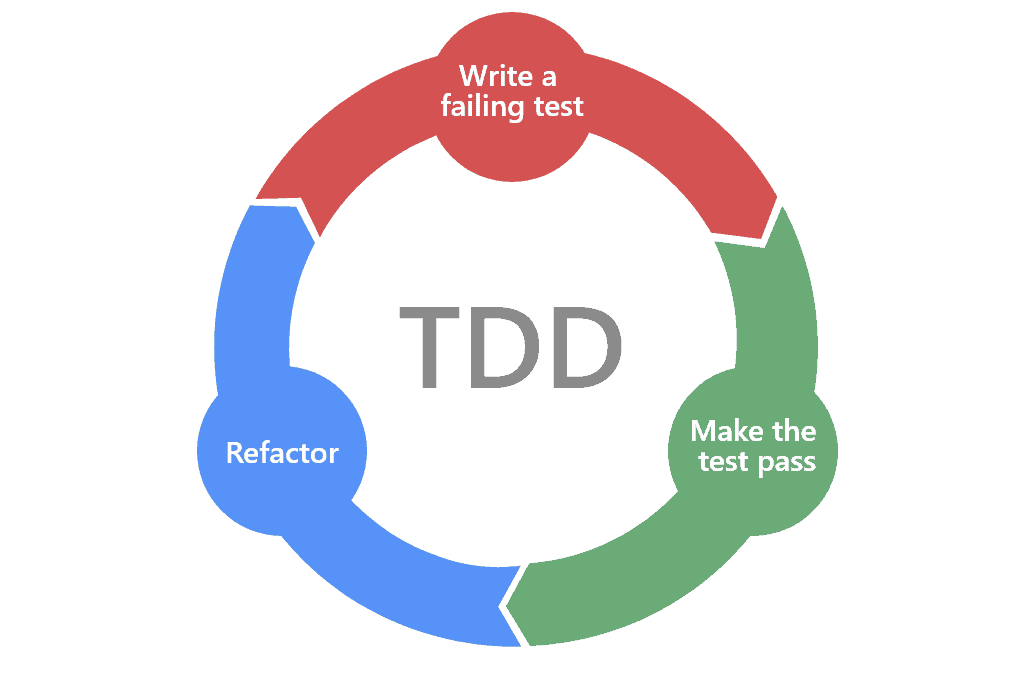
\includegraphics[width=0.68\textwidth]{HerramientasYMetodologias/img/TDD.png}
    \caption{Ciclo iterativo de la metodología TDD (\emph{Test-Driven Development})}
    \label{fig:TDD}
\end{figure}

\clearpage